\chapter{DESIGN AND DEVELOPMENT}

\section{Introduction}
\label{sec:ch3-introduction}

This chapter covers the two central phases of our \ac{DSR} lifecycle: the formalization of the project objectives and the construction of the technological artifact. The chapter is organized in two parts. The first, presented here, details the design and implementation of the \ac{RAG} system, which constitutes the knowledge retrieval layer of the legal assistant. It covers the full data pipeline from acquiring raw legal texts from official Tunisian sources to indexing them in a hybrid vector database ready for semantic retrieval. The second part, to be presented once the training experiments are complete, addresses the domain adaptation of the base language model through supervised fine-tuning on Tunisian legal data.

\section{Definition of Objectives}
\label{sec:ch3-objectives}

The problem analysis conducted in Chapter~I identified two fundamental gaps in E-Tafakna's existing system: the absence of Tunisian legal grounding in the \ac{AI} agents, and an architecture dependent on external cloud services incompatible with the on-premises requirements of \ac{ATI} Tunisie. Addressing these gaps translates into three concrete, measurable objectives that govern the design of the artifact:

\begin{itemize}
    \item \textbf{O1: Domain Adaptation.} Fine-tune a base language model on a curated corpus of Tunisian legal texts, enabling it to understand the specific vocabulary, structure, and reasoning patterns of Tunisian law more accurately than a general-purpose model.

    \item \textbf{O2: Dynamic Knowledge Retrieval.} Design and implement a \ac{RAG} pipeline connecting the language model to an indexed knowledge base of legal documents, grounding responses in retrieved legal evidence at inference time and allowing the knowledge base to be updated independently of model retraining.

    \item \textbf{O3: On-Premises Deployment.} Build and deploy the complete system on \ac{ATI} Tunisie's local infrastructure using open-source tools, ensuring full data sovereignty with no dependency on external \ac{API}s or cloud services at inference time.
\end{itemize}

Table~\ref{tab:objectives-mapping} maps each objective to the problem it addresses and the validation criterion that will be used to assess it in Chapter~IV.

\begin{table}[H]
\centering
\caption{Objectives, Problems Addressed, and Evaluation Criteria}
\label{tab:objectives-mapping}
\renewcommand{\arraystretch}{1.3}
\begin{tabular}{|p{0.8cm}|p{3.5cm}|p{4cm}|p{4cm}|}
\hline
\textbf{ID} & \textbf{Objective} & \textbf{Problem Addressed} & \textbf{Evaluation Criterion} \\
\hline
O1 & Domain Adaptation via Fine-Tuning &
Lack of Tunisian legal knowledge in general-purpose models &
Legal Q\&A accuracy compared to a generic baseline \\
\hline
O2 & Dynamic Retrieval via RAG &
Knowledge bounded by training data; cannot update without retraining &
Retrieval precision on held-out legal queries \\
\hline
O3 & On-Premises Deployment &
Dependency on external cloud \ac{API}s &
Complete inference with zero external calls \\
\hline
\end{tabular}
\end{table}

% ================================================================
% PART I: RAG SYSTEM IMPLEMENTATION
% ================================================================

\needspace{6\baselineskip}
\section{RAG System Architecture}
\label{sec:rag-system-architecture}

\subsection{Overall System Architecture}

The \ac{RAG} system operates around two distinct flows sharing the same data layer. The first is an offline data pipeline responsible for acquiring, processing, and indexing the Tunisian legal corpus. This pipeline runs once at system initialization and is subsequently triggered when new legal texts are published. The second is a query-time flow that handles user queries at runtime: a question is embedded, the vector database is searched for the most semantically relevant legal articles, and the retrieved content is injected into the language model's prompt before generating a response. Both flows run entirely on-premises.

\begin{figure}[H]
\centering
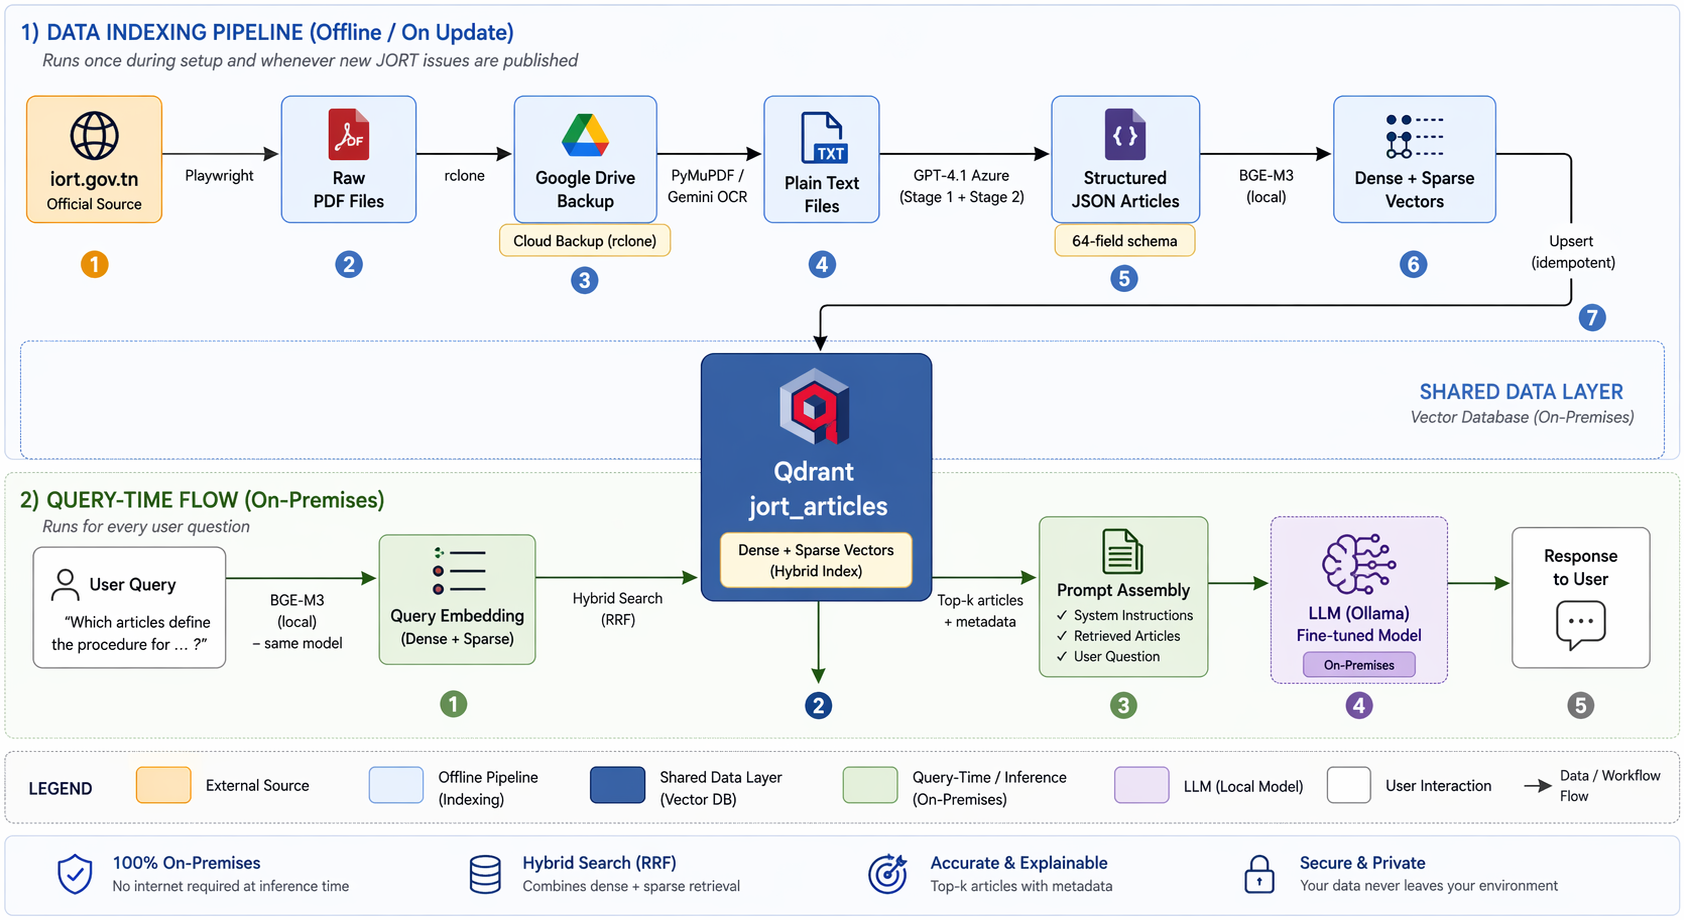
\includegraphics[width=0.95\textwidth]{figures/system_architecture.png}
\caption{Overall Architecture of the Legal AI System}
\label{fig:system-architecture}
\end{figure}

Both flows share the same embedding model and vector database, guaranteeing that the representations used at indexing time are identical to those used at retrieval time. All components run on-premises: no data leaves the local environment at any stage of either flow.

\subsection{Pipeline Data Flow}
\label{subsec:pipeline-dataflow}

The offline pipeline consists of seven sequential phases, each producing structured output consumed by the next. Figure~\ref{fig:bpmn-pipeline} illustrates the complete data flow from raw \ac{PDF} acquisition to a queryable vector database.

\begin{figure}[H]
\centering
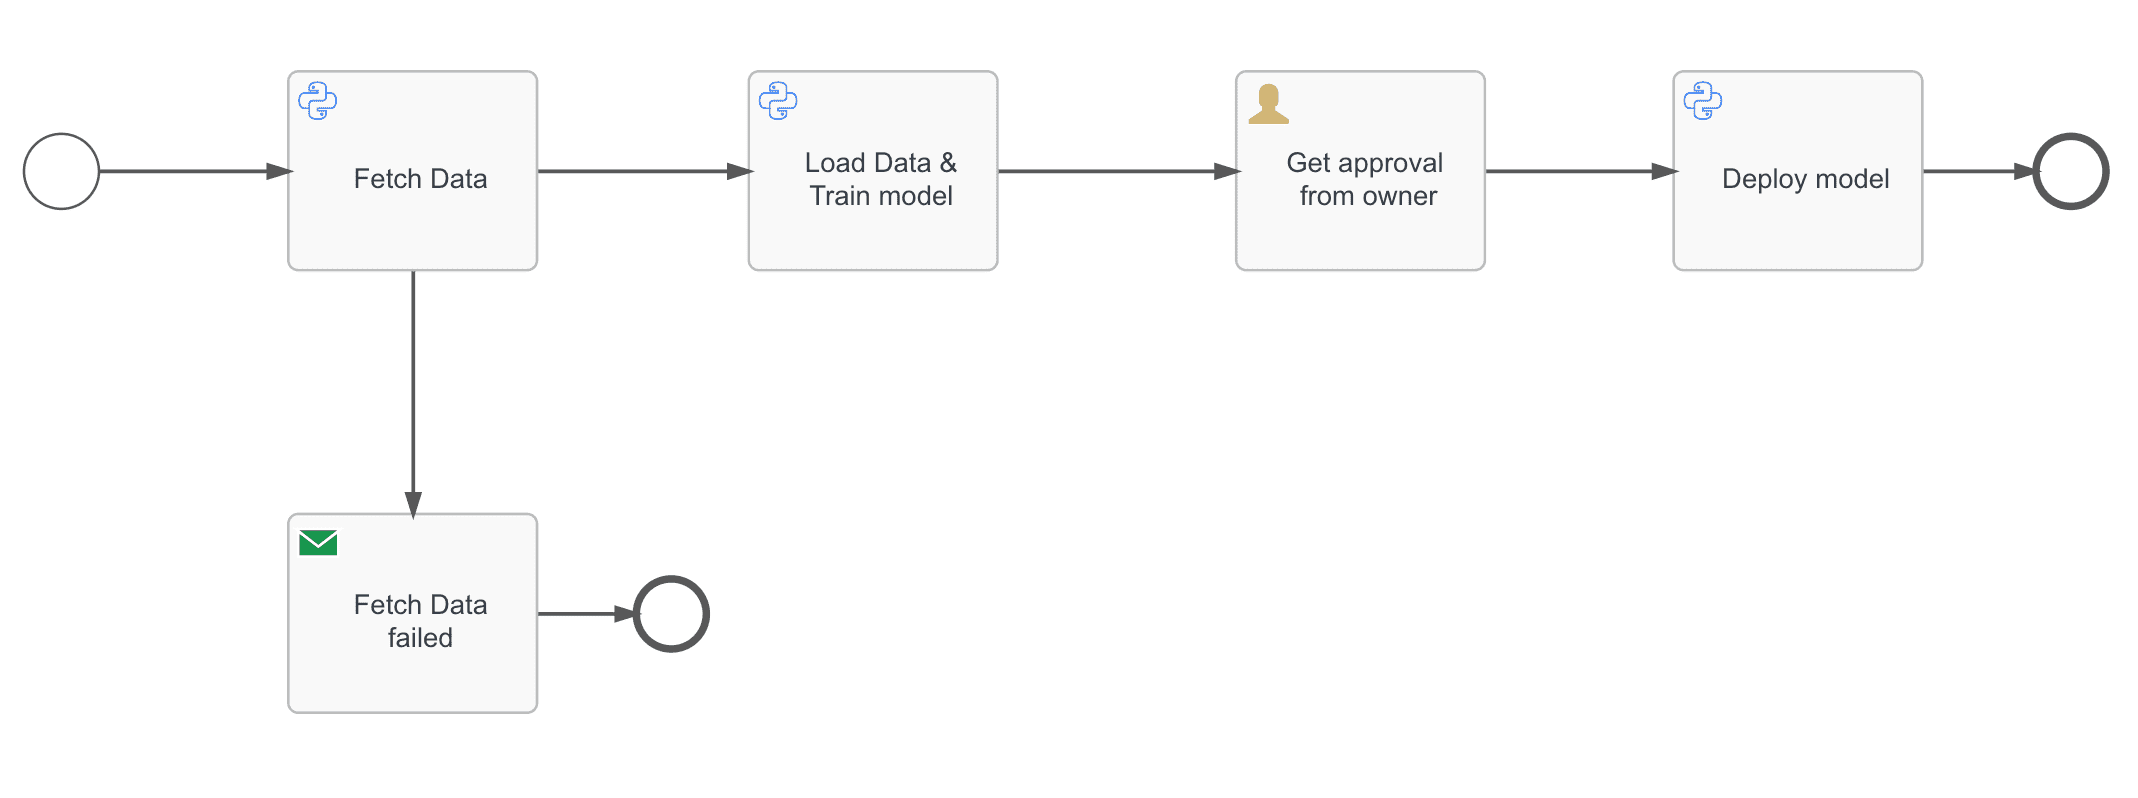
\includegraphics[width=0.95\textwidth]{figures/bpmn_pipeline.png}
\caption{BPMN Diagram of the Offline Data Pipeline}
\label{fig:bpmn-pipeline}
\end{figure}

Table~\ref{tab:pipeline-phases} summarizes each phase, its inputs and outputs, and the key tool responsible for its execution.

\begin{table}[H]
\centering
\caption{Pipeline Phases, Inputs, Outputs, and Key Tools}
\label{tab:pipeline-phases}
\renewcommand{\arraystretch}{1.3}
\begin{tabular}{|p{0.5cm}|p{2.8cm}|p{2.8cm}|p{2.8cm}|p{2.5cm}|}
\hline
\textbf{\#} & \textbf{Phase} & \textbf{Input} & \textbf{Output} & \textbf{Key Tool} \\
\hline
1 & PDF Acquisition & iort.gov.tn & Raw PDFs & Playwright \\
\hline
2 & Cloud Backup & Raw PDFs & Google Drive copy & rclone + n8n \\
\hline
3 & Text Extraction & Raw PDFs & Plain text files & PyMuPDF + Gemini \\
\hline
4 & Article Extraction & Plain text files & Structured JSON & GPT-4.1 (Azure) \\
\hline
5 & Validation & Structured JSON & Validated JSON & Python \\
\hline
6 & Embedding & Validated JSON & Dense + sparse vectors & BAAI/bge-m3 \\
\hline
7 & Vector Storage & Vectors + metadata & Qdrant collection & Qdrant \\
\hline
\end{tabular}
\end{table}

\subsection{Technology Stack}

Table~\ref{tab:tech-stack} presents the complete technology stack organized by functional layer.

\begin{table}[H]
\centering
\caption{Technology Stack by Functional Layer}
\label{tab:tech-stack}
\renewcommand{\arraystretch}{1.3}
\begin{tabular}{|p{3.2cm}|p{3.8cm}|p{5.5cm}|}
\hline
\textbf{Layer} & \textbf{Technology} & \textbf{Role} \\
\hline
Web Scraping & Playwright (Python) \cite{playwright2024docs} & Browser automation for iort.gov.tn \\
\hline
Text Extraction & PyMuPDF \cite{pymupdf2024docs} + Gemini \cite{google2024vertexai} & Digital and scanned \ac{PDF} text extraction \\
\hline
Article Structuring & GPT-4.1 (Azure OpenAI) \cite{microsoft2024azureopenai} & Two-stage semantic article extraction \\
\hline
Embedding & BAAI/bge-m3 \cite{chen2024bgem3} & Bilingual dense and sparse vectorization \\
\hline
Vector Storage & Qdrant (Docker) \cite{qdrant2024docs} & Hybrid semantic and lexical search \\
\hline
API Layer & FastAPI \cite{fastapi2024docs} & HTTP interface for each pipeline phase \\
\hline
Orchestration & n8n (self-hosted) \cite{n8n2024docs} & Automated workflow chaining and monitoring \\
\hline
Development & Python \cite{python2024docs} + VS Code \cite{microsoft2024vscode} & Scripting and pipeline development \\
\hline
\end{tabular}
\end{table}

\section{Legal Corpus Acquisition}
\label{sec:corpus-acquisition}

\subsection{Source: Journal Officiel de la République Tunisienne}
\label{subsec:jort}

The primary source for the legal corpus is the Journal Officiel de la République Tunisienne (JORT), the official gazette of the Tunisian state, published by the government and accessible at iort.gov.tn. The JORT is the authoritative publication for all Tunisian legislation and covers three main sections:

\begin{itemize}
    \item \textbf{Lois, Décrets, Décisions et Avis:} The primary legislative section, containing laws, presidential and governmental decrees, ministerial decisions, and official notices. This section forms the core of the legal corpus.

    \item \textbf{Annonces Légales:} Legal notices covering sharia court decisions, judicial announcements, and commercial registrations.

    \item \textbf{Tribunal Foncier:} Land registry court rulings on property rights and real estate matters.
\end{itemize}

Each section is accessible through both Arabic and French interfaces on the website, yielding six distinct scraping targets. Coverage spans from [START\_YEAR] to [END\_YEAR], producing a corpus of [N] JORT issues and [N] \ac{PDF} documents across all sections.

\subsection{Automated PDF Acquisition}
\label{subsec:scraping}

The JORT website is a legacy application built on the WinDev/WebDev framework and exposes no public \ac{API}. Automated acquisition therefore requires direct browser interaction. We implemented a Python scraping system using Playwright \cite{playwright2024docs}, a browser automation library that drives a Chromium instance to navigate the site, select the target year and issue, and trigger the \ac{PDF} download for each entry.

Each scraping script is fully resumable. Progress is tracked in a checkpoint JSON file that records the download status of every issue as \texttt{downloaded}, \texttt{skipped}, or \texttt{failed}. Re-running the script on a partially completed session safely skips already-downloaded files without duplicating work. Download triggers differ across journal sections, as the site uses different WinDev named anchors and JavaScript calls for each section, requiring section-specific navigation logic.

The scripts are not invoked directly during pipeline execution. Instead, they are exposed through a FastAPI endpoint (\texttt{POST /legal\_extraction/scraping/run}), which launches the scraper as a background job and returns a job identifier for status polling.

\subsection{Cloud Backup}

Downloaded \ac{PDF}s are mirrored to Google Drive using rclone, a command-line utility for syncing local directories to cloud storage. This backup step is triggered automatically after each successful scraping run by the n8n orchestration workflow. The folder tree on Google Drive mirrors the local directory layout, preserving the section and year hierarchy for easy cross-referencing. The backup provides redundancy against local disk failure and a collaborative access point for the raw corpus during the project.

\section{Text Extraction and Article Structuring}
\label{sec:text-structuring}

\subsection{Hybrid PDF-to-Text Conversion}
\label{subsec:hybrid-extraction}

The JORT corpus contains two fundamentally different categories of \ac{PDF}: digitally generated files, where the text is encoded as a selectable text layer, and scanned files, where each page is stored as a rasterized image with no embedded text. These two categories require distinct extraction strategies, applied on a per-page basis.

For each page, a routing decision is made based on two conditions. A page is classified as digital and processed with PyMuPDF \cite{pymupdf2024docs} if it contains more than 50 characters of selectable text and its image content occupies less than 15\% of the page area. Pages that fail either condition are sent to Gemini via Google Vertex AI \cite{google2024vertexai} for \ac{OCR}.

The Gemini model receives a rendered image of the page and is prompted to return the extracted text in a structured format: Arabic tables are preserved as markdown pipe tables with right-to-left column ordering, and non-table content is returned as plain prose. This hybrid routing strategy ensures high-quality extraction across the full diversity of the corpus, combining the speed of direct text layer extraction for the majority of pages with the accuracy of a vision-capable model for scanned content.

The output of this phase is one plain text file per JORT issue, with each page separated by a header marker that preserves page boundary information for downstream parsing.

\subsection{Article-Level Extraction Using GPT-4.1}
\label{subsec:article-extraction}

Converting plain text JORT issues into individually structured legal articles is the most semantically demanding step of the pipeline. Rather than applying a generic text-splitting strategy, we designed a two-stage extraction pipeline powered by GPT-4.1 \cite{microsoft2024azureopenai} that identifies and enriches legal articles as the natural semantic unit of the corpus.

\textbf{Stage 1: Boundary Detection.}
The model receives the full text of a JORT issue and identifies the boundaries of each individual legal article within the document. It returns a raw list of article objects containing the article text, number, title, parent law name, and chapter. This stage operates at the document level, allowing the model to reason about the hierarchical structure of the issue before committing to individual article extractions.

\textbf{Stage 2: Semantic Enrichment.}
Each article identified in Stage 1 is passed back to the model individually for deep enrichment. The model expands each raw article into a rich schema spanning approximately 45 fields across identification, content, legal analysis, and retrieval metadata. Table~\ref{tab:article-schema} presents the key field groups.

\begin{table}[H]
\centering
\caption{Legal Article Schema: Key Field Groups}
\label{tab:article-schema}
\renewcommand{\arraystretch}{1.3}
\begin{tabular}{|p{3.5cm}|p{9cm}|}
\hline
\textbf{Group} & \textbf{Representative Fields} \\
\hline
Identification &
\texttt{jurisdiction}, \texttt{law\_type}, \texttt{law\_number}, \texttt{year}, \texttt{status} \\
\hline
Content &
\texttt{title\_french}, \texttt{title\_arabic}, \texttt{content\_french}, \texttt{content\_arabic} \\
\hline
Summaries &
\texttt{summary\_french}, \texttt{summary\_arabic} \\
\hline
Legal Analysis &
\texttt{keywords}, \texttt{legal\_domains}, \texttt{legal\_concepts}, \texttt{business\_impact} \\
\hline
Structural Flags &
\texttt{has\_obligations}, \texttt{has\_penalties}, \texttt{has\_deadlines}, \texttt{is\_abrogation} \\
\hline
Source &
\texttt{source\_name}, \texttt{source\_date}, \texttt{parent\_document\_id} \\
\hline
Retrieval &
\texttt{embedding\_text} (purpose-built combination of title, content, and metadata) \\
\hline
\end{tabular}
\end{table}

Among these fields, \texttt{embedding\_text} warrants particular attention. Rather than embedding raw article content directly, Phase 4 constructs a dedicated text field that combines the article title, body, key legal concepts, and the parent law name into a single coherent passage. This deliberate construction ensures that the resulting embedding captures both the specific content of the article and its legal context, improving retrieval quality over naive content embedding.

The pipeline includes a fallback chain to handle extraction failures gracefully. If Stage 1 fails after retries, a regular expression (\texttt{Article \textbackslash d+}) identifies article boundaries as a heuristic fallback. If Stage 2 enrichment fails for a specific article, a minimal schema is generated from the raw content with empty enrichment fields, ensuring the pipeline continues without data loss.

\subsection{Why Article-Level Extraction Is Preferable to Generic Chunking}
\label{subsec:chunking-rationale}

As discussed in Chapter~II, the three most common chunking strategies for \ac{RAG} pipelines are fixed-size, recursive, and semantic. For Tunisian legal texts, none of these generic approaches is fully satisfactory. Fixed-size chunking frequently splits articles across chunk boundaries, severing the logical connection between an article's conditions and its obligations. Recursive chunking, while more aware of sentence and paragraph boundaries, remains blind to the hierarchical structure of legal documents and may group unrelated provisions from adjacent articles.

The two-stage GPT-4.1 extraction implements a structurally superior form of semantic chunking, one guided by the actual legal architecture of the document rather than arbitrary size thresholds. Each resulting unit is a complete, self-contained legal article, enriched with metadata fields that enable precise filtering and ranking at retrieval time. In Tunisian legal texts, the article is simultaneously the natural unit of legislative meaning and the natural unit of legal citation, making article-level segmentation the most semantically faithful representation of the corpus.

\section{Embedding and Vector Storage}
\label{sec:embedding-vector}

\subsection{Embedding Model: BAAI/bge-m3}
\label{subsec:bge-m3-embedding}

Each article extracted in the previous phase is converted into a vector representation using BAAI/bge-m3 \cite{chen2024bgem3}, a multilingual embedding model developed by the Beijing Academy of Artificial Intelligence. The model runs entirely on local hardware using the \texttt{FlagEmbedding} Python library, with no external \ac{API} call required at any stage of the embedding process.

For each article, bge-m3 produces two complementary representations from the \texttt{embedding\_text} field in a single encoding pass:

\begin{itemize}
    \item \textbf{Dense vector:} A 1024-dimensional floating-point array encoding the semantic meaning of the text. Dense vectors support approximate nearest-neighbor search and surface results that are semantically related to a query even when the exact phrasing differs.

    \item \textbf{Sparse vector:} A set of token-level lexical weights, stored as a mapping from token identifiers to weight values. Sparse vectors support precise keyword matching, particularly effective for retrieving articles that contain specific legal terms, article numbers, or law references.
\end{itemize}

Both representations are generated alongside all article metadata and persisted to disk before being loaded into the vector database in the subsequent phase. The model operates with 16-bit floating-point precision (\texttt{use\_fp16=True}) to remain within the \ac{VRAM} budget of the available \ac{GPU} while preserving embedding quality.

\subsection{Hybrid Vector Database: Qdrant}
\label{subsec:qdrant-db}

The embeddings and metadata produced in Phase 6 are stored in Qdrant \cite{qdrant2024docs}, an open-source vector database running in a local Docker container. Qdrant was selected over alternatives such as \ac{FAISS} and Chroma for three reasons: its native support for named vector fields enabling hybrid dense and sparse search within a single collection, its production-grade stability under concurrent queries, and its fully self-hosted deployment model that aligns with the on-premises constraints of the project.

The collection, named \texttt{jort\_articles\_v2}, is configured with two named vector fields:

\begin{itemize}
    \item \textbf{dense} (1024 dimensions, cosine distance): supports approximate nearest-neighbor search over the semantic embedding space.
    \item \textbf{sparse} (lexical weights, dot product): supports exact and near-exact keyword matching using the sparse representations produced by bge-m3.
\end{itemize}

At query time, both vector types are searched simultaneously and their result sets are merged using Reciprocal Rank Fusion (RRF), a score combination technique that aggregates rankings from multiple retrieval signals without requiring manual weight calibration. This hybrid approach consistently outperforms either dense or sparse retrieval alone on legal texts, where a user query may match an article semantically (a paraphrased question about contract validity) or lexically (a direct citation such as ``Article 2 du Code des Obligations et des Contrats'').

Ten payload fields are indexed for filtered retrieval, including \texttt{year}, \texttt{law\_type}, \texttt{institution}, \texttt{legal\_domains}, \texttt{has\_obligations}, \texttt{has\_penalties}, \texttt{is\_abrogation}, and \texttt{status}. These filters allow the retrieval layer to scope a search to a specific legal category or time period without scanning the full collection. Insertion into the database is idempotent: each article carries a stable identifier assigned at embedding time, and Qdrant's upsert operation inserts a new record or overwrites an existing one with the same identifier, making it safe to re-run the pipeline on the same corpus.

\subsection{Retrieval at Inference Time}
\label{subsec:inference-retrieval}

When a user submits a query to the legal assistant, the retrieval process mirrors the indexing process. The query text is embedded using the same bge-m3 model, producing a dense and a sparse vector. These vectors are submitted to Qdrant as a hybrid search request, and the top-$k$ articles are returned based on the RRF-fused score.

The retrieved articles are injected into the language model's prompt alongside the original query. Each article contributes its content in the language matching the query (Arabic or French) together with its source metadata: the law name, article number, and publication date. This metadata allows the model to produce responses that include proper legal citations, making each answer directly verifiable against the original JORT source. The value of $k$ is treated as a tunable hyperparameter and will be optimized during the evaluation phase described in Chapter~IV.

\section{Pipeline Orchestration}
\label{sec:pipeline-orchestration}

\subsection{FastAPI Service Layer}
\label{subsec:fastapi-service}

Each of the seven pipeline phases is exposed as an asynchronous \ac{HTTP} endpoint through a FastAPI \cite{fastapi2024docs} application. This design allows any phase to be triggered independently, monitored, and retried without rerunning the full pipeline. All endpoints follow a consistent job-based pattern:

\begin{itemize}
    \item A \texttt{POST} request to the phase-specific endpoint starts a background job and returns a job identifier.
    \item A \texttt{GET} request to \texttt{/legal\_extraction/status/\{job\_id\}} returns the current status (\texttt{queued}, \texttt{running}, \texttt{done}, or \texttt{failed}), along with timing information and any associated error message.
\end{itemize}

This uniform interface decouples the orchestration logic from the implementation details of each phase, making it straightforward to replace or extend a phase without modifying the workflow that drives it.

\subsection{n8n Workflow Automation}
\label{subsec:n8n-automation}

The n8n \cite{n8n2024docs} workflow connects the seven pipeline phases into a single automated sequence. n8n is a self-hosted, open-source workflow automation platform that communicates with external services through configurable \ac{HTTP} request nodes. Its self-hosted deployment model ensures that no data or credentials are transmitted to any external service, in line with the project's data sovereignty requirements.

The workflow follows a consistent pattern for each phase, as illustrated in Figure~\ref{fig:n8n-workflow}:

\begin{enumerate}
    \item \textbf{Trigger:} An \ac{HTTP} node calls the FastAPI endpoint for the current phase and retrieves the job identifier.
    \item \textbf{Notify:} A notification node sends an immediate message confirming the job has started.
    \item \textbf{Poll:} A Wait node pauses for 30 to 60 seconds, followed by an \ac{HTTP} node that polls the status endpoint.
    \item \textbf{Branch:} A Switch node routes execution based on the returned status. A \texttt{done} status advances to the next phase; a \texttt{failed} or \texttt{error} status triggers an error notification and halts the pipeline; a \texttt{running} or \texttt{queued} status loops back to the Wait node.
    \item \textbf{Guard:} An IF node at the beginning of each subsequent phase verifies the success of the previous one before triggering the next job.
\end{enumerate}

\begin{figure}[H]
\centering
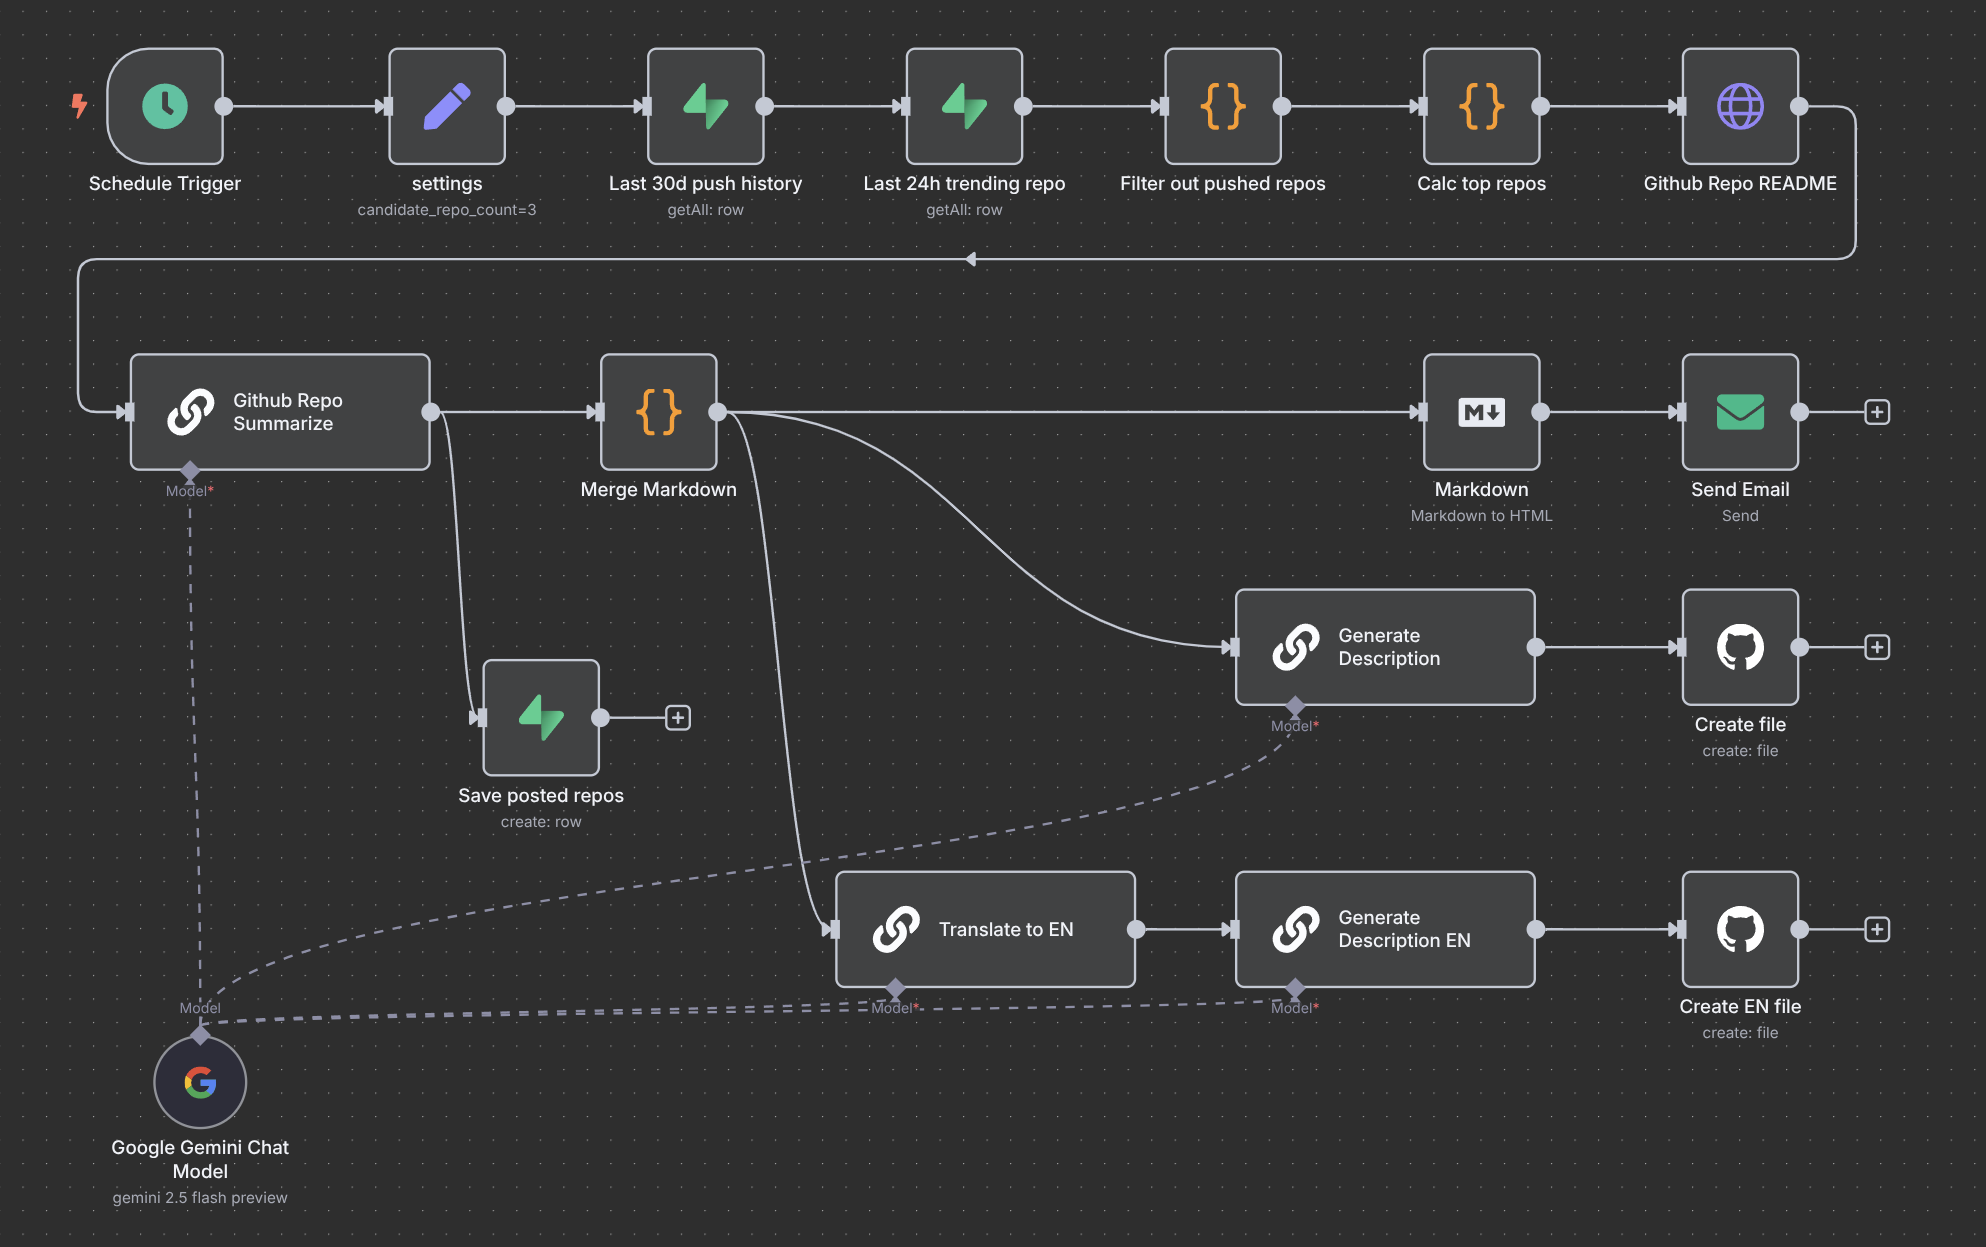
\includegraphics[width=0.95\textwidth]{figures/n8n_workflow.png}
\caption{n8n Workflow: Automated Pipeline Orchestration \cite{n8n2024docs}}
\label{fig:n8n-workflow}
\end{figure}

The complete workflow consists of 43 nodes covering all seven phases, with notifications at each transition point for real-time monitoring without requiring active observation of the pipeline execution.

\section{Conclusion}

This chapter presented the design and implementation of the \ac{RAG} system forming the knowledge retrieval layer of the legal assistant. Beginning from the official Tunisian legal gazette, the pipeline acquires, processes, and structures the full JORT corpus into individually enriched legal articles, converts them into bilingual dense and sparse vector representations using bge-m3, and stores them in a hybrid Qdrant collection optimized for legal retrieval. The complete pipeline is orchestrated through an automated n8n workflow backed by a FastAPI service layer, running entirely on-premises with no dependency on external services at inference time.

The following part of this chapter, to be presented once the training experiments are complete, addresses the supervised fine-tuning of the base language model on a synthesized Tunisian legal dataset.
